\chapter{\label{Method}Machine Learning}
\epigraph{Machine Learning can be defined as the process of inducing intelligence into a system or machine without explicit programming}{-Andrew NG}
The machine learning (ML) subset of artificial intelligence (AI) allows computer applications to become more accurate by predicting outcomes without being explicitly programmed(not providing commands on each step).  The algorithms used by the machines depend on historical or past data as input to predict new outputs. We are surrounded by numerous applications of machine learning in our daily life such as image recognition software's, speech recognition(Voice search, voice dialing), Predictive analytics(Predicting whether a transaction is fraudulent or legitimate, Whether mail is spam or not), etc.

Machine learning is very important nowadays as it provides an overview of trends in customer behavior and operational business patterns, also supports the development of new products. The most common examples can be taken from today's leading tech companies, such as Facebook, Google, and car rental companies, Uber, which use machine learning as a central part of their operations. For handling a large amount of data, machine learning has always been an efficient method. This chapter discusses the basic concept of machine learning and how neural network functions, which are more efficient and productive compared to traditional workflow.[\cite{25-26}]


\section{Types of Machine Learning:}
There are four basic approaches for machine learning: supervised learning, unsupervised learning, semi-supervised learning, and reinforcement learning. The type of algorithm that will be used depends on what type of data they want to predict.
\subsection{Supervised Learning}
In this type of machine learning, we supply algorithms with labeled training datasets and define the variables that we want the algorithm to assess for correlations and the outputs. 
Both the input and the output of the algorithm have been already specified. Supervised machine learning requires getting trained with the algorithm on both labeled inputs and desired outputs. A simple example would be the classification of datasets.
\subsection{Unsupervised learning:}
This type of machine learning involves algorithms that train on unlabeled datasets. The algorithm scans through datasets looking for any meaningful connection without any human intervention. The data on which algorithms train as well as the predict the output is predetermined. For example, unsupervised learning is used for Google news categorization, visual perception tasks such as image recognition, anomaly detection, classifying customers, etc.

\subsection{Semi-supervised learning:}
This approach to machine learning involves a mix of both the previous types of the dataset; that is algorithm is trained upon the combination of the labeled and unlabeled dataset.  In this type of algorithm, the programmer just needs to cluster similar data using an unsupervised learning algorithm and further use the existing labeled data to label the rest of the unlabeled data. A few practical examples of this type of learning are speech analysis, internet content classifications, and protein sequence classification.


\subsection{Reinforcement learning: }
Data scientists usually use reinforcement learning to teach a machine to complete a multistep process( based on the rewarding behaviors/ or pushing the undesired one ) for which there is a clearly defined set of rules. In the reinforcement learning decision is dependent on the output of the previous input sequence, so we provide labels to sequences of dependent decisions. For example, chess games or a sitting cat, the cat will only get food when she starts to walk.\\

A brief summary of how machine learning consists can be summarized from this tree diagram,
% \textbf{Add examples to each of the learning}
\resizebox{\linewidth}{!}{%
\begin{center}
    \begin{forest}
  [Machine Learning
    [Supervised \\ Learning
     [Classification 
       [Binary \\ classification]
       [Multi \\classification]
     ]
     [Regression
       [Regression \\ modeling
         [\textit{Ensembling}]
       ]
     ]
    ]
    [Unsupervised \\ Learning
      [Clustering
      [K-means Clustering]
      ]
      [Anomaly detection
        % [V$'$
        %   [V
        %     [\textit{is}]
        %   ]
        %   [AP
        %     [Deg
        %       [\textit{extremely}]
        %     ]
        %     [A$'$
        %       [A
        %         [\textit{straightforward}]
        %       ]
        %       [CP
        %         [\textit{to wield}, roof]
        %       ]
        %     ]
        %   ]
        % ]
      ]
    ]
    [semi-supervised\\ learning
    ]
    [reinforcement \\learning
    ]
  ]
\end{forest}
\end{center}
}%

\section{Evaluating models}
In machine learning, the ultimate goal is to achieve models that generalize, i.e., that perform well on never-before-seen data, and overfitting is the central obstacle. To do this, splitting the available data is very crucial. Training, validation, and testing are the partitions  
needed, so during the training phase, the model trains with the training data and test with the validation data, and when the model is ready, it is tested one last time with the test data, briefly explained by \autoref{fig:my_label_09876} \\
\begin{figure}[H]
    \centering
    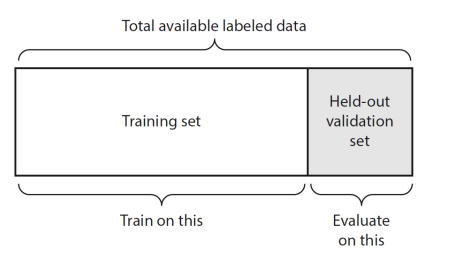
\includegraphics[scale=0.6]{ml__12.png}
    \caption{Splitting data to be used in the training phase. Image source: [Chollet, 2017]}
    \label{fig:my_label_09876}
\end{figure}
The reason why three (and not two) datasets are used is that tuning in the model configuration is required. The parameters that can be tuned in a machine learning model are called hyperparameters. Hyperparameter values can be changed to control the learning process. Meanwhile, the value of other parameters, like node weights, are derived by training and cannot be adjusted. Hyperparameter tuning is done with the feedback of the model performance in the validation data and further applied under an unseen test dataset. This is a basic approach for each machine learning model, and we will apply the same over the neural network model in the next section.

%%%%%%%%%%%%%%%%%%%%%%%%%%%%%%%%%%%%%%%%%%%%%%%%%%%%%%DNNNNNNNNNNNNNDNNNDNNNDNNNNDNNDNNNDNNDNDNNDNDNNDNDNNNDNNNNDNNNDNDNDNDNDNDNDNDNDNDNNDNDNDNDNNDND
\section{Deep Neural Network}
Machine learning works very efficiently on numerous problems but sometimes fails to excel in a few specific cases, which appears very easy for humans. For example, classifying an image as a cat or dog or distinguishing audio clips as a male or female voice,etc\dots The machine fails to identify this type of problem of image classification or video segregation and other unstructured data types, which are easy for us. There come to the idea of a deep neural network(DNN), where the idea is to mimic the human brain's biological process, which is composed of billions of neurons connected to each other and to adapt and learn new things\cite{23-25}. \\ 


A simplified version of Deep Neural Network can be represented as a hierarchical (layered) structure of neurons (compared with the neurons in the human brain) with connections to other neurons. These neurons pass a message or signal to other neurons based on the received input and form a complex network system that learns with some feedback mechanism. The following diagram(\autoref{fig:my_label_hu}) represents an 'N' layered Deep Neural Network.\\

\begin{figure}[H]
    \centering
    \includegraphics[scale=0.4]{1_ML_report.png}
    \caption{A Deep Neural Network with N hidden layers}
    \label{fig:my_label_hu}
\end{figure}
The input data is provided to the neurons into the first layer (not hidden), which subsequently provides an output to the neurons within the next layer and so on and finally provides the final output. These outputs might be a prediction such as Yes or No (just as we represent in probability). Each layer can consist of one or many neurons, and each of them will be computed with the help of a small function, i.e., activation function. The activation function takes the signal from the previous layers and passes it further to the next connected neurons. There is a threshold value corresponding to each activation function, where the output is passed when it is above the threshold value; else, it gets ignored. The connection between two neurons of successive layers always passes with an associated weight. \\
 
 The weights have a very important role to play in the correct prediction from the model. This weight defines the influence of the input on the output for each layer. We provide initial weight to the model randomly, but during the training, these weights get updated iteratively to learn to predict a suitable output.\\
 In a neural network, the initial weights would be provided by us as a random number, but during the model training, these weights are updated iteratively by themselves to learn to predict a correct output. The network also depends on the learning mechanism (optimizer), which helps the neural network to update its weights (that were randomly initialized) to a more suitable weight that aids in the correct prediction of the outcome.  To update its weight for the connections, the mathematical algorithm used is called backpropagation. The iteration of the process several times, with more and more data, helps the model to update its weights appropriately. By iterating the process several times, with the help of more data, the networks update the weights appropriately to create a system where the system can take a decision for predicting output based on rules which the model created for itself with the help of weights and connections\cite{22-23}.\\


Deep learning is efficient to work with a large amount of data which has made it popular in the last few years; a few of the popular choices for the frameworks of deep learning in python are:-\\
 \begin{itemize}
     \item Low-level frameworks 
         \begin{itemize}
             \item TensorFlow
             \item MxNet
             \item PyTorch
         \end{itemize}
      \item High-level frameworks
         \begin{itemize}
             \item Keras (uses TensorFlow as a backend)
              \item Gluon (uses mxnet as a backend)
         \end{itemize}
 \end{itemize}

Schematically, a neural network(unit, node) layer can be represented as in below \autoref{fig:my_label_3}. 
\begin{figure}[H]
    \centering
    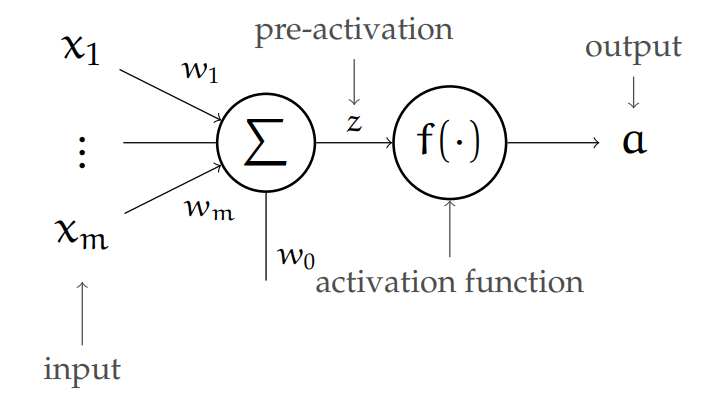
\includegraphics[scale =0.5]{Figures/ml__1.png}
    \caption{Basic structure of a neural network}
    \label{fig:my_label_3}
\end{figure}




The function representing the neural network can be expressed as:

\begin{equation}\label{eq:eq1}
a= f(z) = f(\sum_{j=1}^{j=m} x_jw_j +w_0) = f(w^T x+w_0)
\end{equation}
A non-linear function of an input vector x $\in \mathbb{R}^m$ note to a single output value  a $\in$R . It is parameterized by a vector of weights  $(w_1, w_2,....w_m)\in \mathbb{R}^m$  and an offset or threshold  $w_0\in \mathbb{R}^m$ . In order for the neuron to be non-linear, we also specify an activation function  $f:\mathbb{R} \to \mathbb{R}$ , which can be the f(x)=x(linear function), or can also be any other non linear function, such as ReLU, tanh, etc., which is differentiable. 
\\
Before thinking about a whole network,let us consider how to train a single unit. \\
Given a loss function L(guess, actual) and a dataset $\{(x^{(1)},y^{(1)}),.....,(x^{(n)},y^{(n)})\}$, we can do (stochastic) gradient descent, adjusting the weights w, $w_0$ to minimize the equation 

\begin{equation} \label{eq:eq2}
    J(W, W_0) = \sum_{i=1} ^n L(f(x^{(i)}:W),y^{(i)})
\end{equation}
where f is the output of our neural net for a given input.

% \textbf{Provide example here :linear logistic classifiers (LLC)
% with NLL loss and regressors with quadratic loss! The activation function for the LLC is
% f(x) = $\sigma$(x) and for linear regression it is simply f(x) = x. \\
% Just for a single neuron, imagine for some reason, that we decide to use activation function f(z) = $e^z$ and loss function $L(g, a) = (g-a)^2$. Derive a gradient descent update for w and $w_0$.}

%%%%%%%%%%%%%%%%%%DO from here%%%%%%%%%%%%%%%%%%%
\subsection{Networks}


Now, we’ll try to train the network with stacking multiple neurons together to form a network. A neural network in general takes input $x \in \mathbb{R}^m$ and generates an output $\alpha \in \mathbb{R}^n $.  It is constructed with the help of multiple neurons; the inputs of each neuron might be elements of x and/or outputs of other neurons. The outputs are generated by n output units.
Here, for the training of data, we will only consider feed-forward networks. In a feed-forward network, we can think of the network as defining a function-call graph that is acyclic. For the simplicity in software and analysis, we usually organize networks into layers. A \textbf{layer} can be defined as a group of neurons which are connected to each other parallelly (as in \autoref{fig:my_label_hu}): The input of a hidden layer depends on the output of previous layer(hidden or input layer); and the output from the layers are input to the neurons in the subsequent next layer. We will start to describe about the model with a single layer and further go on to the case of multiple layers.

\subsubsection{Single-layer}
A layer is a set of units that, as we have just described, are not connected to each other. The
layer is called fully connected if, as in the diagram below, the inputs to each unit in the layer
are the same. A layer has input x $\in \mathbb{R}^m$ and output (also known as activation) $\alpha \in \mathbb{R}^n$
\begin{figure}[H]
    \centering
    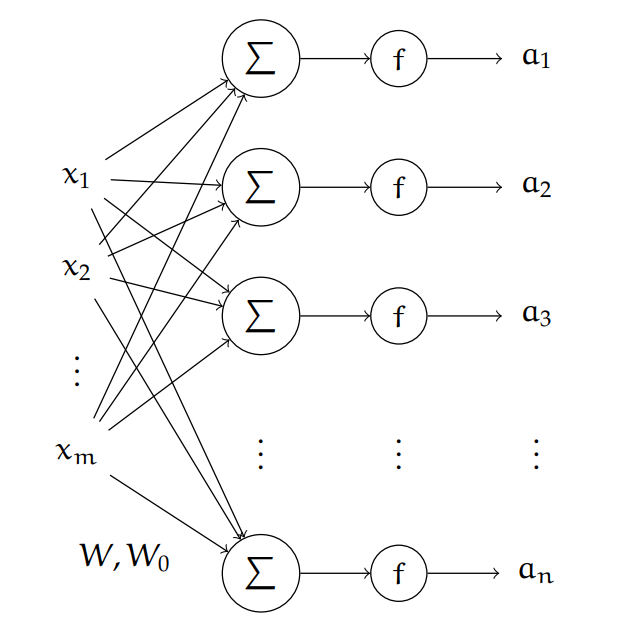
\includegraphics[scale=0.3]{Figures/ml_2.png}
    % \caption{Caption}
    \label{fig:my_label}
\end{figure}
Since each unit layer has a vector of weights and a single offset, we can consider the weights of
the whole layer as a matrix, W, and the collection of all the offsets as a vector $W_0$. If we
have m inputs, n units, and n outputs, then,
\begin{itemize}
    \item  W is an m $\times$ n matrix
     \item $W_0$ is an n$\times$  1 column vector,
     \item X, the input, is an m $\times$  1 column vector,
     \item Z = W$^T$X + $W_0$, the pre-activation, is an n$\times$  1 column vector,
\end{itemize}
and the output vector will be\\
\begin{equation*}
    A = f(Z) = f(W^Tx +W_0)
\end{equation*}

\subsubsection{Many layers}

A single neural network generally consists of multiple layers, where the output of the previous layer feeds as input to the next layer..\\
 We will use l to name a layer and 
let $m^l$ be the  number of inputs to the layer and $n^l$ be the number of outputs from the layer. Then, $W^l$ and $W^l _0$ are of shape $m^l \times n^l$, respectively. Let $f^l$ be the activation
function of layer  $ \ell$ . Then, the pre-activation outputs are the $n^l \times$ 1 vector, such that,
\begin{equation*}
    Z^l = {W^l}^T A^{l-1} + W_0^l
\end{equation*}
and the activation function outputs are simply the $n^l \times 1$ vector
\begin{equation*}
    A^l = f^l(Z^l)
\end{equation*}
We will use this structural diagram to organize our algorithmic thinking and implementation different parameters in deep neural network.
\begin{figure}[H]
    \centering
    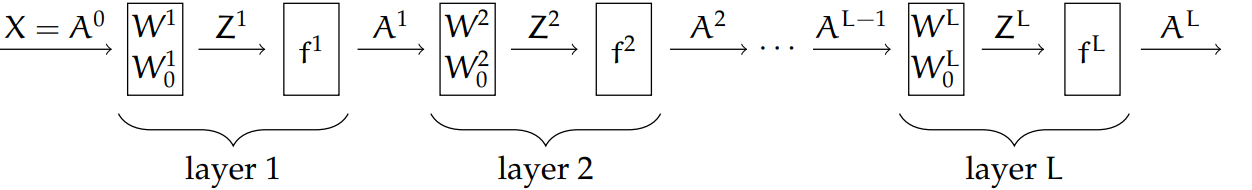
\includegraphics[scale=0.3]{Figures/ml__3.png}
    % \caption{Caption}
    \label{fig:my_label}
\end{figure}

As we saw here how a model of neural network function, the training and output from any model depends on the type of non linear functions Z, i.e. activation function we use in between the layers. Now, the question arises, how many types of activation functions are there?, and how we choose which one will be suitable for our model? We will addresses all these issues over the next section.

\subsection{ Activation function}
\label{subsection:Activationfunction}
There are three types of neural networks activation functions:
\subsubsection{Binary Step Function}
Binary step function depends on a threshold value which decides whether a neuron should be activated or not. This can be represented using the equation \autoref{eq:2}

\begin{equation} \label{eq:2}
   f(x) =  \begin{cases} 
      0 for x < 0 \\
      1 for x \geq 0 
   \end{cases}
\end{equation}
The output of the equation can be represented graphically as,
\begin{figure}[H]
    \centering
    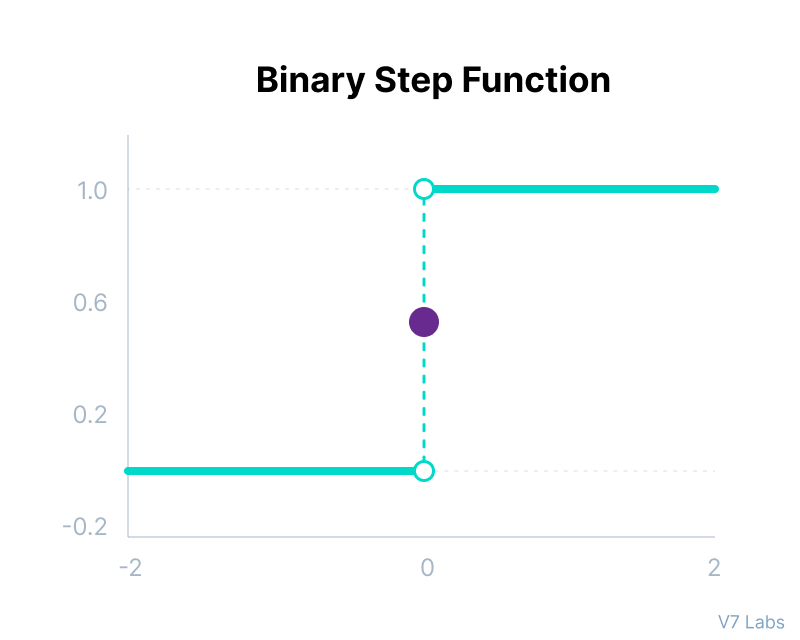
\includegraphics[scale=0.2]{Act_1.jpg}
    % \caption{Caption}
    \label{fig:my_label}
\end{figure}
The binary activation function is not always useful; a few of its limitations are:
\begin{itemize}
    \item We cannot use this activation function to provide us an output of multiclass problems, as it has only two labels of output.
    \item The gradient of the step function is zero, which causes a restriction in the back propagation process.
\end{itemize}

 
\subsubsection{Linear Activation Function}
Also known as identity Function, i.e. it can be represented using equation, and fig. below,
\begin{equation}
    f(x) = x
\end{equation}

\begin{figure}[H]
    \centering
    \includegraphics[scale=0.2]{Act_2.jpg}
    % \caption{Caption}
    \label{fig:my_label_02wwe}
\end{figure}

However, a linear activation function also has these two major problems :

\begin{itemize}
    \item It’s impossible to use back propagation as the gradient of the function is always a constant and has no relation with the input x.
    \item After use of linear activation function, without having dependence on a number of layers, the last layer will still be a linear function of the first layer. A linear activation function turns the neural network model into just one layer, which leads to model collapse.
\end{itemize}

 
\subsubsection{Non-Linear Activation Functions}

Non-linear activation functions solve the above limitations possessed by both linear activation functions and binary activation function as the derivative are possible and also related to the inputs, thus backpropogation are allowed here.

Few non-linear activation functions are:-\\
\textbf{Sigmoid / Logistic Activation Function}\\
Input is any real value(i.e. x $\in$ $\mathbb{R}$)and outputs $\in$ [0,1].\\
Mathematically, it can be represented as:\\
\begin{equation}
    f(x) = \frac{1}{1+e^{-x}}
\end{equation}
The output of the above equation is,
\begin{figure}[H]
    \centering
    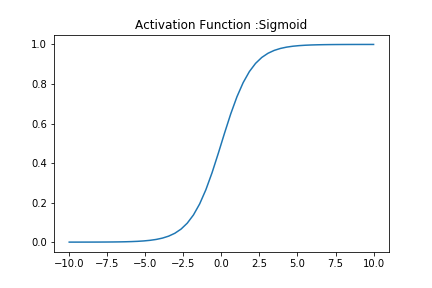
\includegraphics{Figures/sigmoid.png}
    % \caption{Caption}
    \label{fig:my_label}
\end{figure}

\textbf{Tanh Function}\\
Tanh function is very similar to the sigmoid/logistic activation function, with only difference in the output range of -1 to 1. 
Mathematically, it can be represented as;
\begin{equation}
    f(x) = \frac{e^x - e^{-x}}{e^x + e^{-x}}
\end{equation}
And, graphically, it can be represented as,\\
\begin{figure}[H]
    \centering
    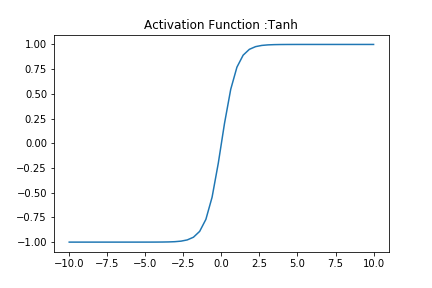
\includegraphics{Figures/Tanh.png}
    % \caption{Caption}
    \label{fig:my_label}
\end{figure}


Tanh activation function gives advantages as the output of the tanh activation function is Zero centered; thus, we can easily map the output values as strongly negative, neutral, or strongly positive. Another advantage is that the value of the hidden layers in a neural network has its values  between -1 to 1, and the mean for the hidden layer comes out to be 0 or very close to it. Therefore, it helps in centering the data and makes learning for the next layer much easier.

\textbf{ReLU} \\
ReLU stands for Rectified Linear Unit. ReLU has a derivative function, despite seems like linear function. It allows backpropagation and also simultaneously making it computationally efficient. The ReLU function does not activate all the neurons at the same time. The neurons get deactivated when its output is less than 0, that is,
\begin{equation}
    f(x) = max(0,x) = \begin{cases} 
      0 & z < 0 \\
      z & otherwise 
   \end{cases}
\end{equation}

\begin{figure}[H]
    \centering
    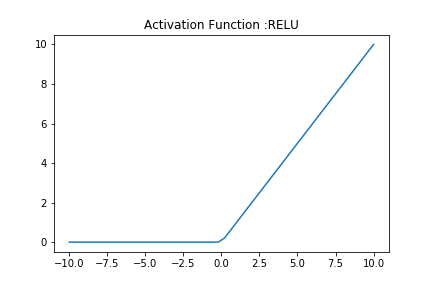
\includegraphics{Figures/RELU.png}
    % \caption{Caption}
    \label{fig:my_label}
\end{figure}


It is the most commonly used activation  function due to following unique features. Since ReLU activation function activate only a certain number of neurons, and it help them to do computation efficiently  in comparison to the sigmoid and tanh functions. The ReLU activation function also increase or decrease the rate of convergence towards global minimum of the loss function due to its linear, non saturating property[\cite{21}].

\textbf{Softmax}\\
It is used to calculate the relative probabilities. Like sigmoid activation function, the SoftMax function also returns the probability of each class. \\
It is the most commonly used activation function for the last or output layer of the neural network in the case of multi-class classification. \\
Mathematically it can be represented as:
\begin{equation}
    softmax(z_i) = \frac{exp(z_i)}{\sum_j exp(z_j)}
\end{equation}
\begin{figure}[H]
    \centering
    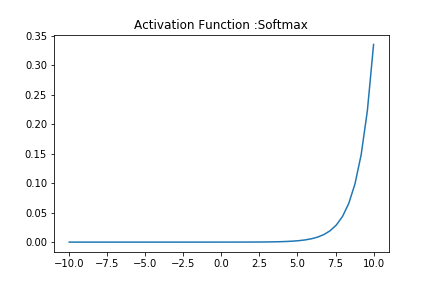
\includegraphics{Figures/softmax.png}
    % \caption{Caption}
    \label{fig:my_label}
\end{figure}
Here, we saw a few common activation functions, but how we can choose activation function for the given problem? 

\subsubsection{How to choose activation function for Hidden Layers}
The choice of activation function in between the layers depends on the type of problem we have, as it is summarized in the tree below.
 \begin{center}
    \begin{forest}
      [
      Network type?
       [Multilayer Perceptron
        [ReLU \\ Activation]
       ]
       [Convolutional Neural Net
        [ReLU \\ Activation]
         ]
        
       [Recurrent Neural Net
       [sigmoid Activation]
       [Tanh Activation]
       ]
      ] 
    %   [Multi-class\\ cross-Entropy \\Loss \\ Functions
    %   [Multi-class\\ Cross-Entropy\\ Loss]
    %   [Sparse Multiclass \\cross-Entropy \\loss]
    %   [Kullback\\ Leibler\\ Divergence \\Loss]
    %   ]
      
    \end{forest}
 \end{center}



\subsubsection{How to choose activation function for output layers}
% \begin{figure}[H]
%     \centering
%     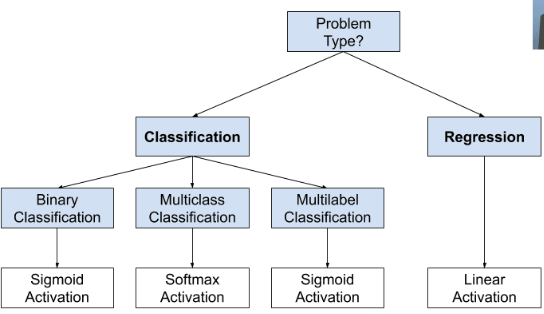
\includegraphics[scale=0.5]{Figures/ml__4.png}
%     % \caption{Caption}
%     \label{fig:my_label}
% \end{figure}
The activation function used in the final layer of the neural network depends on what type of output we need and on the type of prediction problem that we are solving, which can be summarized from the tree below.
\begin{itemize}
    \item \textbf{Regression}: one node, Linear Activation
    \item \textbf{Binary Classification}:one node per class, Softmax Activation
    \item \textbf{Multiclass Classification}:One node per class, softmax activation
    \item \textbf{Multilabel Classification}: One node per class, sigmoid activation
\end{itemize}

 \begin{center}
    \begin{forest}
      [
      Problem type?
       [Classification
        [Binary \\ Classification
         [Sigmoid Activation]
        ] 
        [Multiclass \\ Classification
         [Softmax Activation]
         ]
        [Multilabel \\ Classification
        [Sigmoid Activation]
        ]
       ]
       [Regression
       [Linear Activation]
       ]
    %   [Multi-class\\ cross-Entropy \\Loss \\ Functions
    %   [Multi-class\\ Cross-Entropy\\ Loss]
    %   [Sparse Multiclass \\cross-Entropy \\loss]
    %   [Kullback\\ Leibler\\ Divergence \\Loss]
    %   ]
      ]
    \end{forest}
 \end{center}

% \begin{figure}
%     \centering
%     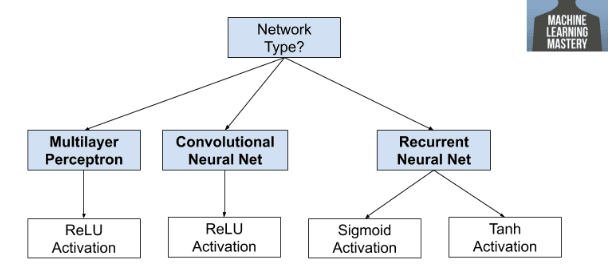
\includegraphics[scale=0.5]{Figures/ml__5.png}
%     % \caption{Caption}
%     \label{fig:my_label}
% \end{figure}















% Source
% \url{https://machinelearningmastery.com/choose-an-activation-function-for-deep-learning/}
% \url{https://www.v7labs.com/blog/neural-networks-activation-functions}
% ReLUs are especially common in internal (“hidden”) layers, and sigmoid activations are
% common for the output for binary classification and softmax for multi-class classification.(\url{https://openlearninglibrary.mit.edu/assets/courseware/v1/9c36c444e5df10eef7ce4d052e4a2ed1/asset-v1:MITx+6.036+1T2019+type@asset+block/notes_chapter_Neural_Networks.pdf}
\section{Training of Neural Network}



\subsection{Error backpropagation}
We will train our neural networks using gradient descent methods. It’s possible to use batch gradient descent, in which we sum up the gradient over all the points or stochastic gradient descent (SGD), where we take a small step with respect to the gradient after considering a single point at a time[\cite{23}].
% \textbf{Include theorem from} \url{https://openlearninglibrary.mit.edu/assets/courseware/v1/d81d9ec0bd142738b069ce601382fdb7/asset-v1:MITx+6.036+1T2019+type@asset+block/notes_chapter_Gradient_Descent.pdf}\\

we will always compute the gradient of the loss function with respect
to the weights for a particular value of (x, y). That tells us how much change is needed in the
weights, in order to reduce the loss experienced on this particular training. Let us understand with this example.\\
First, let’s us calculate and observe how the loss depends on the weights in the final layer, $W^L$ remembering
that our output is $A^L$, and using the shorthand loss to stand for Loss((f(x; W), y) which
is equal to Loss($A^L$, y), and finally that $A^L$ = $f^L$($Z^L$) and $Z^L$ = ${W^L}^T$ $A^{L-1}$, we can apply the chain  rule as:
\begin{figure}[H]
    \centering
    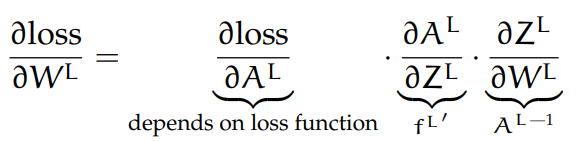
\includegraphics[scale = 0.3]{Figures/ml__6.png}
    % \caption{Caption}
    \label{fig:my_label}
\end{figure}
Here, we need to be little careful with the dimensions, and here we can note that it is true for any $ \ell$, including $ \ell$ = L\\
\begin{figure}[H]
    \centering
    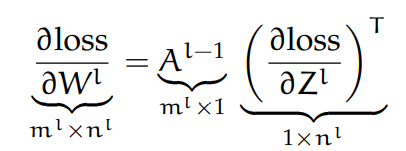
\includegraphics[scale=0.3]{Figures/ml__7.png}
    % \caption{Caption}
    % \label{fig:my_label}
\end{figure}
If we can repeatedly apply the chain rule, we will obtain this expression for the gradient of the loss with respect to the pre-activation function in the first layer:
\begin{figure}[H]
    \centering
    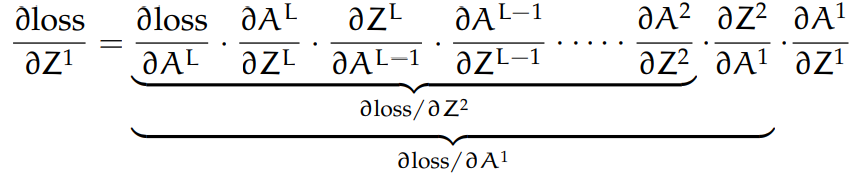
\includegraphics[scale=0.3]{Figures/ml__8.png}
    % \caption{Caption}
    \label{fig:my_label}
\end{figure}


Here,
\begin{itemize}
    \item $\frac{\partial loss}{\partial A^L}$ is $n^L \times 1$ and depends on the particular loss function you are using.
    \item $\frac{\partial Z^l}{\partial A^{l-1}}$ is $m^L \times n^L$ and is just $W^l$
    \item $\frac{\partial A^l}{\partial Z^l}$ is $n^L \times n^L$. Each element $\alpha_i ^l = f^l(z_i ^l)$. This means that $\frac{\partial \alpha_i ^l}{\partial z_j ^l}$ = 0 whenever i$\neq$ j. So, the off-diagonal elements of $\frac{\partial A^l}{\partial Z^l}$ are all 0, and the diagonal elements are $\frac{\partial \alpha_i ^l}{\partial z_j ^l}$= ${f^l}^'(z_j ^l)$
\end{itemize}
We can write the above equation as,
\begin{figure}[H]
    \centering
    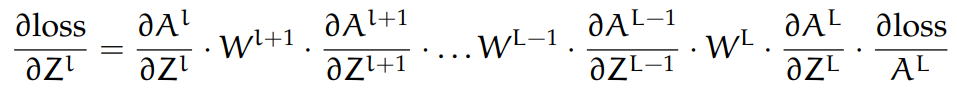
\includegraphics[scale=0.3]{Figures/ml__09.png}
    % \caption{Caption}
    \label{fig:my_label}
\end{figure}

This general process is called error back-propagation. The general idea is that we will do a forward
pass to compute all the $\alpha$ and z values at all the layers. Then, we can start work backward direction and compute the gradient of the loss with respect
to the weights in every layer, starting at last layer L and going back to layer 1, in this way model can update its weight, as can be shown below,\\
\begin{figure}[H]
    \centering
    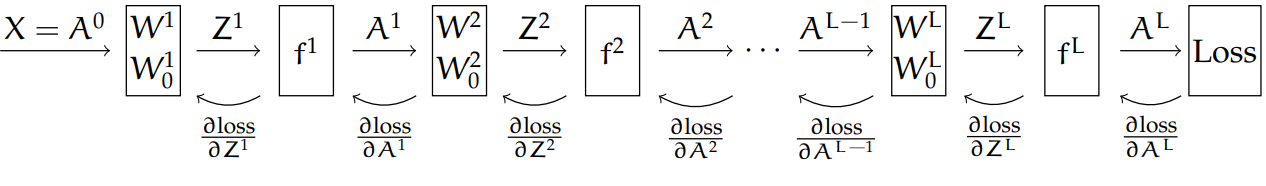
\includegraphics[scale=0.3]{Figures/ml__10.png}
    % \caption{Caption}
    \label{fig:my_label}
\end{figure}




Now, How we can do stochastic gradient descent training on a feed-forward neural network. This is the pseudo code to apply stochastic gradient descent,

% \begin{algorithm}
% \caption{\textit{SGD-NEURAL-NET(D_n,T, L, ($m^1$, ...$m^L$), ($f^1$,......,$f^L$))}}\label{alg:cap}
% \begin{algorithmic}
% \for {l=1 to L}
% \State $W_{ij} ^l ~ Gaussian(0, \frac{1}{m^l})$
% % \ $y = x^n$
% % \State $y \gets 1$
% % \State $X \gets x$
% % \State $N \gets n$
% % \While{$N \neq 0$}
% % \If{$N$ is even}
% %     \State $X \gets X \times X$
% %     \State $N \gets \frac{N}{2}$  \Comment{This is a comment}
% % \ElsIf{$N$ is odd}
% %     \State $y \gets y \times X$
% %     \State $N \gets N - 1$
% % \EndIf
% % \EndWhile
% \end{algorithmic}
% \end{algorithm}

\begin{lstlisting}[language=Python]
def SGD(f, theta0, alpha, num_iters):
    """
      Arguments:
      f -- the function to optimize, it takes a single argument
            and yield two outputs, a cost and the gradient
            with respect to the arguments
      theta0 -- the initial point to start SGD from
      num_iters -- total iterations to run SGD for
      Return:
      theta -- the parameter value after SGD finishes
    """
    start_iter = 0
    theta = theta0
    for iter in xrange(start_iter + 1, num_iters + 1):
        _, grad = f(theta)
  
        # there is NO dot product ! return theta
        theta = theta - (alpha * grad)
\end{lstlisting}



\section{Loss functions }
Now, the choice of a loss function for a particular problem is a very tedious task. We can take a rough idea about the loss function from this tree,\\
\resizebox{\linewidth}{!}{%
 \begin{center}
    \begin{forest}
      [
      Loss Function
       [Regression \\Loss\\ functions
        [Mean \\ Squared \\Error loss]
        [Mean\\ Squared \\Logarithmic \\Error loss]
        [Mean\\ absolute\\ Error\\ Loss]
       ]
       [Binary \\Classification\\ Loss \\Functions
       [Binary \\Cross- Entropy]
       [Hinge\\ Loss]
       [Squared\\ Hinge Loss]
       ]
       [Multi-class\\ cross-Entropy \\Loss \\ Functions
       [Multi-class\\ Cross-Entropy\\ Loss]
       [Sparse Multiclass \\cross-Entropy \\loss]
       [Kullback\\ Leibler\\ Divergence \\Loss]
       ]
      ]
    \end{forest}
 \end{center}
}

Like activation function, loss function also take different assumptions about the range of inputs it will take depending on the type of problem in hand. While designing the model of neural network, it become important to make things to fit well together. As, in particular, we will think about matching loss function with activation function of the last layer, $f^L$. This hypothesis can be infer from the table below, \autoref{tab:my_label_12}.\\
\begin{table}[h]
    \centering
    \begin{tabular}{ccc} \hline
   \textit{   Loss }  & \textit{ $f^L$} & \textit{Comments}\\ \hline
      squared   &  Linear &  --\\
      hinge  &  Linear &  for "maximum-margin" classification\\
      NLL &   Sigmoid &   negative log likelihood loss. Useful to \\ 
      &    &       train classification problem with C classes.\\
      NLLM & softmax & -- \\
      
    \end{tabular}
    \caption{Few loss functions corresponding to the last layer/ output layer activation function. There are many different types of the loss function following the kind of problem, whether it belongs to classification or regressions. }
    \label{tab:my_label_12}
\end{table}
There are also other loss function we have used to make our model better, such as "BinaryCrossentropy", "CategoricalCrossentropy", and
"SparseCategoricalCrossentropy" belonging to probabilistic losses. Also, "mean\_squared\_error", "mean\_absolute\_error", and "MeanSquaredError" belonging to regression losses.
 
\subsubsection{Two-class classification and log likelihood}

% For classification, the natural loss function is 0-1 loss, but we have already discussed the
% fact that it’s very inconvenient for gradient-based learning because its derivative is discontinuous. \\
For binary classification problems, which are useful in separation of signal and background, Hinge loss gives us another way, to make a smoother objective, penalizing the margins of the labeled points relative to the separator. The hinge loss is defined to be
\begin{equation*}
    L_h(guess, actual) = max(1-guess.actual,0)
\end{equation*}
when actual $\in$ \{+1, -1\}
 Using hinge loss, together with a squarednorm regularizer, forces the learning process to try and find a separator that has the
maximum margin relative to the data set. This optimization set-up is called a \textbf{support vector machine}. It was popular because it has a quadratic form that makes SVM to get easily optimized.

\subsubsection{Multi-class classification and log likelihood}
Multi-class classification with total of K classes, where the training label is represented with the one-hot vector $y = [y_1,...., y_k]^T$, where $y_k$= 1 if the example is of class k.Assume that our network uses softmax as the activation function (Which is most commomly used activation function for multi classification) in the last layer, so that the output is
$\alpha = [\alpha_1,....,\alpha_k]^T$, which represents a probability
distribution over the K possible classes. Then, the probability that our network predicts
the correct class for this example is $\Pi_{k=1} ^N \alpha_k ^y$ and the log of the probability that it is correct is $\sum_{k=1} ^k y_k \log \alpha_k$,so
\begin{equation*}
    L(guess, actual) = - \sum_{k=1} ^K actual_k.log(guess_k)
\end{equation*}





\section{Optimizing neural network parameters}
As neural networks consists of many parameters, our ultimate goal to minimize the loss function. The optimization can be done with help of standard gradient-descent softwares, but here, we can take advantages of the structure of the loss functions to improve optimization. The structure of loss function as a sum over terms, one training data point, help us to consider stochastic gradient methods. In this section, we will try to consider some alternative strategies for organizing training, and also to make easier to handle the step-size parameter.\\


\subsection{Batches}

Lets us assume we have an objective function of the form\\
\begin{equation*}
    J(W) = \sum_{i=1} ^n L(h(x^{(i)};W),y^{(i)})
\end{equation*}
where h is the function computed by a neural network, and W stands for all the weight
matrices and vectors in the network.\\
When we perform batch gradient descent, we use the update rule \\
\begin{equation*}
    W := W-\eta \nabla_W J(W), 
\end{equation*}
which is equivalent to 
\begin{equation*}
     W := W-\eta \nabla_W \sum_{i=1} ^n L(h(x^{(i)};W),y^{(i)})
\end{equation*}
Thefore, we add up the gradient of loss after each training point, with respect to W, and then take a step in the negative direction of the gradient to minimize the loss.\\


A more effective strategy for optimization is to take “average” between batch and stochastic gradient descent by using mini-batches. For a mini-batch of size k, we select k distinct data points uniformly at random from the data set and do the weight update based just on their contributions to the gradient.
\begin{equation*}
    W \leftarrow W-\eta \nabla_W \sum_{i=1} ^n L(h(x^{(i)};W),y^{(i)})
\end{equation*}
Most neural network software packages are set up to do mini-batches\cite{25}.\\

To select k unique data points at random from a large dataset is computationally difficult. An alternative strategy, if we have an efficient procedure for randomly shuffling the data set (or randomly shuffling a list of indices into the data set) is to operate
in a loop, roughly as follows:\\
\begin{algorithm}
\caption{\textit{MINI-BATCH-SGD(NN, data, k)}}\label{alg:cap}
\begin{algorithmic}
\State $n = length(data)$
\While{not done:}
     \State $RANDOM-SHUFFLE(data)$
     \For {i=1 to $\frac{n}{k}$}
           \State $BATCH-GRADIENT-UPDATE(NN,data[(i-1)k:ik])$
% \Require $n \geq 0$
% \Ensure $y = x^n$
% \State $y \gets 1$
% \State $X \gets x$
% \State $N \gets n$
% \While{$N \neq 0$}
% \If{$N$ is even}
%     \State $X \gets X \times X$
%     \State $N \gets \frac{N}{2}$  \Comment{This is a comment}
% \ElsIf{$N$ is odd}
%     \State $y \gets y \times X$
%     \State $N \gets N - 1$
% \EndIf
% \EndWhile
\end{algorithmic}
\end{algorithm}
then, we can easily divide the dataset into k mini batches.

\subsection{ Adaptive stepsize}

Picking the value for $\eta$ is difficult and time-consuming. As our networks become deep (with increase in the numbers of layers) we can find that magnitude of the gradient of the loss with respect the weights in the last layer,$\frac{\partial loss}{\partial W_L}$,may have significant differences from the gradient of the loss with respect to the weights in the first layer $\frac{\partial loss}{\partial W_1}$.\\

The output gradient is further multiplied by all the weight matrices of the network and is “fed
back” through all the derivatives of the activation functions. This can lead to a general problem
of \textbf{exploding or vanishing gradients}, in which the back-propagated gradient is either too big
or small.

\subsubsection{Running averages}


It is a computation strategy for estimating a weighted average for a sequence of data. Let us take data sequence be $\alpha_1, \alpha_2,......;$ then we define a sequence of running average values, $A_0, A_1, A_2,....$ using the equations
\begin{equation*}
      A_0 = 0
\end{equation*}
\begin{equation*}
         A_t = \gamma_t A_{t-1} + (1-\gamma_t)\alpha_t
\end{equation*}
where $\gamma_t$ $\in$ (0,1). If $\gamma_t$ is a constant, then this is a moving average, in which
\begin{equation*}
         A_T = \gamma A_{T-1} + (1-\gamma)\alpha_T
\end{equation*}
\begin{equation*}
       = \gamma(\gamma A_{T-2} +(1-\gamma)\alpha_{T-1}) +(1-\gamma)\alpha_T
\end{equation*}
\begin{equation*}
     = \sum_{t=0} ^T \gamma^{T-t}(1-\gamma)\alpha_t
\end{equation*}
So, you can see that inputs $\alpha_t$ closer to the end of the sequence have more effect on $A_t$ than early inputs.\\


\subsubsection{Momentum}
 we can use this method a bit like running averages to describe strategies for computing $\eta$. The simplest method is momentum, in which we try to “average” recent gradient updates so that if they have been bouncing oscillating in some direction, then we at least take out that component of the motion. For momentum, we have\\
\begin{equation*}
      V_0 = 0
\end{equation*}
\begin{equation*}
         V_t = \gamma V_{t-1} + \eta \nabla_W J (W_{t-1})
\end{equation*}
\begin{equation*}
         W_t =  W_{t-1} - V_t
\end{equation*}
This does not look like an adaptive step-size method. But, if we let
$\eta = \eta'(1-\gamma)$ then the rule looks exactly like doing an update with step size $\eta'$ on a moving average of the gradients with parameter $\gamma$:
\begin{equation*}
    M_0 = 0
\end{equation*}
\begin{equation*}
           M_t = \gamma M_{t-1} + (1-\gamma) \nabla_W J (W_{t-1})
\end{equation*}
\begin{equation*}
         W_t =  W_{t-1} - \eta'M_t
\end{equation*}

\begin{figure}[H]
    \centering
    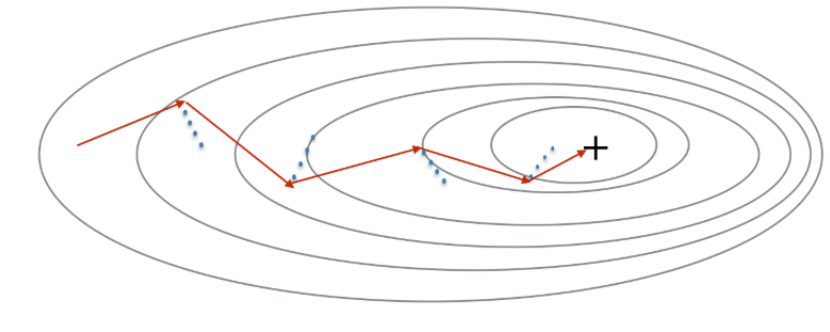
\includegraphics[scale=0.3]{Figures/ml__11.png}
    \caption{The red arrows show the change in the value of weight after one step of mini-batch gradient descent with use of momentum. The blue points show about the direction of the gradient with respect to
the mini-batch at each step. The Momentum smooths the path taken towards the local
minimum and further leads to faster convergence.\cite{21},\cite{25}}
    \label{fig:my_label}
\end{figure}

\subsubsection{Adadelta}
Here the idea is to take larger steps in parts of the space where J(W) get nearly flat (as there are no risks of taking too larger step due to the gradient being large) and smaller steps when it is steep. We’ll apply this idea to each weight, and at the end we obtain a method called adadelta. 
Even, here our weight are indexed by layers including input and output unit, just let $W_j$ be any weight in the network\\
\begin{equation*}
    g_{t,j} = \nabla_W J (W_{t-1})_j
\end{equation*}
\begin{equation*}
       G_{t,j }= \gamma G_{t-1, j} + (1-\gamma) g_{t,j}^2
\end{equation*}
\begin{equation*}
    W_{t,j} = W_{t-1,j}- \frac{\eta}{\sqrt{G_{t,j}+\epsilon}}g_{t,j}
\end{equation*}
% The sequence $G_{t,j}$ is a moving average of the square of the jth component of the gradient.
% We square it in order to be insensitive to the sign—we want to know whether the magnitude is big or small. Then, we perform a gradient update to weight j, but divide the step
% size by $\sqrt{G_{t,j}+\epsilon}$,which is larger when the surface is steeper in direction j at point $W_{t-1}$ in weight space; this means that the step size will be smaller when it’s steep and larger when
% it’s flat.

\subsubsection{Adam}

Adam has become the most common and default method of managing step sizes neural networks. The moving averages of the gradient
and squared gradient, which estimates the mean and variance of the gradient for weight j:
\begin{equation*}
     g_{t,j} = \nabla_W J (W_{t-1})_j
\end{equation*}
\begin{equation*}
        m_{t,j} = B_1 m_{t-1,j} + (1-B_1) g_{t,j}
\end{equation*}
\begin{equation*}
        v_{t,j} = B_2 v_{t-1,j} + (1-B_2) g_{t,j}^2
\end{equation*}

If we initialize $m_0$ = $v_0$ = 0, then there will always be bias(slightly too small). So we will correct the bias by defining,
\begin{equation*}
    \hat{m}_{t,j} = \frac{m_{t,j}}{1-B_1^t}
\end{equation*}
\begin{equation*}
    \hat{v}_{t,j} = \frac{v_{t,j}}{1-B_2^t}
\end{equation*}
\begin{equation*}
    W_{t,j} = W_{t-1, j} - \frac{\eta}{\sqrt{ \hat{v}_{t,j}+\epsilon}}\hat{m}_{t,j} 
\end{equation*}
Adam did not have a huge effect on the result after making small changes in the model, which makes it an efficient method.

\section{Regularization}

Till now, we have only discussed how we can optimize loss on our training data. As discussed before, the risk of overfitting is still persistent. This overfitting problem can be rectified with the help of increasing our data size, which is the case nowadays where the deep neural network uses large data size. Nonetheless, there are several strategies for regularizing a neural network, and sometimes they can be important. This can be done using the implementation of early stopping, where the idea is train on the training set, and on every epochs, (pass through the whole training set, or possibly more frequently), evaluate the loss of the current W on a validation set. Here, it is observed that the loss on the training set goes down fairly consistently with each number of iteration, and the loss on the validation set will initially decrease, but then begin to increase
again. Once we observe that the validation loss is systematically increasing, we can stop training the model and return the weights that had the lowest validation error.\\

Another simple method is to penalize the norm of all the weights,This method is known as weight decay,
\begin{equation*}
    J(W) = \sum_{i=1}^n Loss(NN(x^{(i)}), y^{(i)};W) + \lambda ||W||^2
\end{equation*}
we end up with an update of the form\\
\begin{equation*}
    W_t = W_{t-1}(1-\lambda_\eta) - \eta (\nabla_W Loss(NN(x^{(i)}), y^{(i)};W_{t-1}))
\end{equation*}

This rule has the form of first “decaying” $W_{t-1}$ by a factor of (1 -$\lambda \eta$) and then taking a gradient step.\\
Other few methods are:-

% \subsection{Methods related to ridge regression}
% Early stopping is the easiest to implement and is in fairly common use. The idea is
% to train on your training set, but at every epoch (pass through the whole training set, or
% possibly more frequently), evaluate the loss of the current W on a validation set. It will
% generally be the case that the loss on the training set goes down fairly consistently with
% each iteration, the loss on the validation set will initially decrease, but then begin to increase
% again. Once you see that the validation loss is systematically increasing, you can stop
% training and return the weights that had the lowest validation error.\\
% Another common strategy is to simply penalize the norm of all the weights,This method is known as weight decay, because when we take the gradient of the objective
% \begin{equation*}
%     J(W) = \sum_{i=1}^n Loss(NN(x^{(i)}), y^{(i)};W) + \lambda ||W||^2
% \end{equation*}
% we end up with an update of the form\\
% \begin{equation*}
%     W_t = W_{t-1}(1-\lambda_\eta) - \eta (\nabla_W Loss(NN(x^{(i)}), y^{(i)};W_{t-1}))
% \end{equation*}

% This rule has the form of first “decaying” $W_{t-1}$ by a factor of (1 -$\lambda \eta$) and then taking a gradient step.


\subsection{Dropout}

The contains a simple idea, it suggest rather than perturbing the data every time we train, we will make changes in the
network. Here, we will randomly, from each dataset, after selecting a unit layer prohibit them from participating  in the training. Therefore, all of the units will have to take a 
kind of overall responsibility for getting the answer right, and will not be able to rely
on any small subset of the weights to do all the necessary computation. This tends also to
make the network more robust to data perturbations.\\
When we are done training and want to use the network to make predictions, we multiply all weights by p to achieve the same average activation levels. In the forward pass during training, we let\\
\begin{equation}
    \alpha^l = f(z^l) * d^l
\end{equation}
where * denotes component-wise product and $d^l$ is a vector of 0’s and 1’s drawn randomly
with probability p. The backwards pass depends on $\alpha^l$ so we do not need to make any
further changes to the algorithm.
Another modern alternative method to dropout, is batch normalization.\\
\subsection{Batch Normalization}

Here, idea is when training is done with mini-batches, the idea is to standardize the input values for each mini-batch, subtracting off the mean and dividing by the standard deviation of each input dimension. This gives us similar effect to adding noise and dropout. Each mini-batch of data ends up getting mildly perturbed, which prevents the network from exploiting very particular values of the data points.\\
% So, when training with mini-batches, the idea is to standardize the input values for each mini-batch, subtracting off the mean and dividing by the standard deviation of each input dimension. This Batch normalization ends up having a regularizing effect for similar reasons that adding noise and dropout do: each mini-batch of data ends up being mildly perturbed, which prevents the network from exploiting very particular values of the data points.\\


\section{ROC Curve}
Another metric tom measure the output is the Receiver Operating Characteristic (ROC) curve output after training, defined with respect to
a given class \textit{C}. Given a point x and model that outputs a P(C|x) probability that x belongs to the class C. Given T , a threshold, x belongs to C if and only if P(C|x) $\geq$ T . If T = 1, a point is labeled as belonging to class, C only if the model is 100\% sure. If T = 0, every point is labeled as belonging to the class C\\
Each value of the threshold T generates a point (False Positive, True Positive) and, then, the ROC curve is the curve formed by going through T = 0 to T = 1. A good model will have a curve that increases quickly from 0 to 1, the different ROC curve depending over output can be seen in \autoref{fig:my_label-2}
\begin{figure}[H]
    \centering
    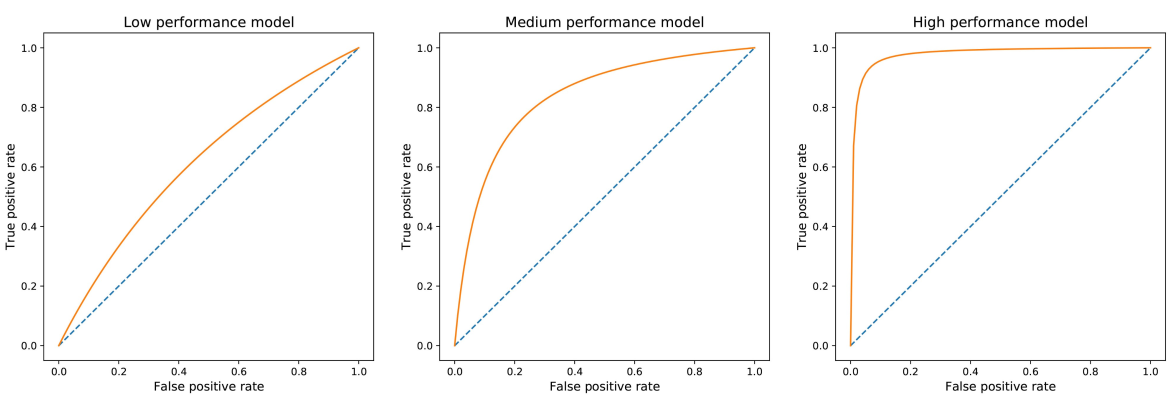
\includegraphics[scale=0.3]{13__ml.png}
    \caption{ROC curves depending on the effectiveness of the model}
    \label{fig:my_label-2}
\end{figure}











%     \textbf{(Maths part may be excluded)}



% 1. \url{https://openlearninglibrary.mit.edu/assets/courseware/v1/9c36c444e5df10eef7ce4d052e4a2ed1/asset-v1:MITx+6.036+1T2019+type@asset+block/notes_chapter_Neural_Networks.pdf}

% \url{https://www.mygreatlearning.com/blog/types-of-neural-networks/}
% \url{MIT lecturre from where you have learnt}






























































































\setcounter{equation}{0}
\setcounter{table}{0}
\setcounter{figure}{0}
%\baselineskip 24pt
